\documentclass[12pt,a4paper]{article}
\usepackage[T1]{fontenc}
\usepackage[utf8]{inputenc}
\usepackage{lmodern}
\usepackage[a4paper,margin=25mm]{geometry}
\usepackage{amsmath,amssymb,amsthm,mathtools}
\usepackage{microtype}
\usepackage{graphicx}
\usepackage{booktabs,tabularx,array}
\usepackage{enumitem}
\usepackage{xcolor}
\usepackage{xurl}
\usepackage[unicode,colorlinks=true,linkcolor=blue!45!black,
 citecolor=blue!45!black,urlcolor=blue!45!black,
 pdftitle={Arithmetic Lower Bounds for the Time Complexity of the Hypervolume Indicator and Klee Measure Problem through the Permanent},
 pdfauthor={Michael T.M. Emmerich},
 pdfkeywords={hypervolume indicator, Klee measure problem, permanent, arithmetic complexity, CC BY 4.0},
 pdfsubject={Reduction from the permanent to hypervolume and Klee measure; conditional arithmetic lower bounds}]{hyperref}
\pagestyle{plain}
\setlength{\parskip}{0.25em}
\setlength{\emergencystretch}{2em}
\setlist{itemsep=0.25em,topsep=0.4em}
\newtheorem{theorem}{Theorem}[section]
\newtheorem{lemma}[theorem]{Lemma}
\newtheorem{proposition}[theorem]{Proposition}
\newtheorem{corollary}[theorem]{Corollary}
\theoremstyle{definition}
\newtheorem{definition}[theorem]{Definition}
\theoremstyle{remark}
\newtheorem{remark}[theorem]{Remark}
\newcommand{\R}{\mathbb R}
\newcommand{\Q}{\mathbb Q}
\newcommand{\F}{\mathbb F}
\newcommand{\HV}{\operatorname{HV}}
\newcommand{\Mag}{\operatorname{Mag}}
\newcommand{\per}{\operatorname{per}}
\newcommand{\VP}{\mathrm{VP}}
\newcommand{\VNP}{\mathrm{VNP}}
\newcommand{\bits}{\{0,1\}}
\newcommand{\one}{\mathbf 1}
\newcommand{\conf}{\mathcal C_r}
\newcommand{\matchings}{\mathcal M_r}
\newcommand{\size}{\mathsf L}
\DeclareMathOperator{\supp}{supp}

\title{Arithmetic Lower Bounds for the\\
Time Complexity of the Hypervolume Indicator\\
and Klee Measure Problem\\
through the Permanent}
\author{Michael T.M. Emmerich\thanks{\textcopyright\ 2026 Michael T.M. Emmerich.
Licensed under \href{https://creativecommons.org/licenses/by/4.0/}{CC BY 4.0}.}\\[0.35em]
\normalsize Faculty of Information Technology\\
\normalsize University of Jyv\"askyl\"a}
\date{26 November 2026}

\begin{document}
\maketitle

\begin{abstract}
The Hypervolume Indicator measures the volume of a union of
axis-aligned boxes that share a reference corner. The Klee Measure
Problem permits arbitrary axis-aligned boxes. We study the difficulty
of computing these volumes exactly when both the number of boxes and
the dimension are allowed to grow.

The connection with the permanent is made through matchings. For an
$r\times r$ matrix with positive entries, we construct $r^2(r-1)$
anchored boxes in $r^2$ dimensions. The boxes cover the cells that
represent selections of entries containing a row or column conflict.
The uncovered part of an enclosing box therefore represents all
matchings, including those that are not perfect. A parameter $t$
records the size of each matching. The uncovered volume is then a
polynomial in $t$, whose coefficient of $t^r$ is the permanent.
Interpolation recovers this coefficient from $r+1$ exact hypervolume
evaluations with polynomial additional arithmetic work.

This reduction is unconditional. It shows that polynomial-size
arithmetic circuits for the constructed hypervolume family would give
polynomial-size circuits for the permanent. Hence, \emph{if
$\VP_{\R}\ne\VNP_{\R}$}, no such circuit family exists. The same
obstruction applies to exact Klee-measure computation in the stated
arithmetic model, because every anchored instance is also a
Klee-measure instance. The result concerns growing dimension and does
not determine the best running time for a fixed number of objectives.

We relate the construction to earlier counting and algebraic results,
give the reverse reduction for rational inputs in the bit model, and
derive exact connections with ordinary $\ell_1$ magnitude. The recent
$\VP\ne\VNP$ announcement remains a preprint \cite{Claude2026};
our lower-bound conclusions remain conditional.
\end{abstract}

\section{Introduction}
\label{sec:models}

In two dimensions, the Klee Measure Problem asks for the area covered
by finitely many axis-aligned rectangles. A point covered by several
rectangles contributes to the area only once. In higher dimensions,
rectangles are replaced by boxes and area by volume.

The Hypervolume Indicator is a special case. All boxes have one common
corner, called the reference point. For maximization, each opposite
corner is an objective vector, and the union is the region dominated
by at least one of these vectors. Figure~\ref{fig:boxes} shows both
constructions. Their similarity is useful: an algorithm for arbitrary
boxes also applies to anchored boxes.

In multiobjective optimization, this volume can be used to compare
finite sets of objective vectors. The common reference point gives
their unions more structure than arbitrary collections of boxes. It is
therefore natural to ask whether that structure permits exact volume
computation with polynomial cost in both the number of vectors and the
number of objectives. This question motivates the present paper.

\begin{figure}[htbp]
\centering
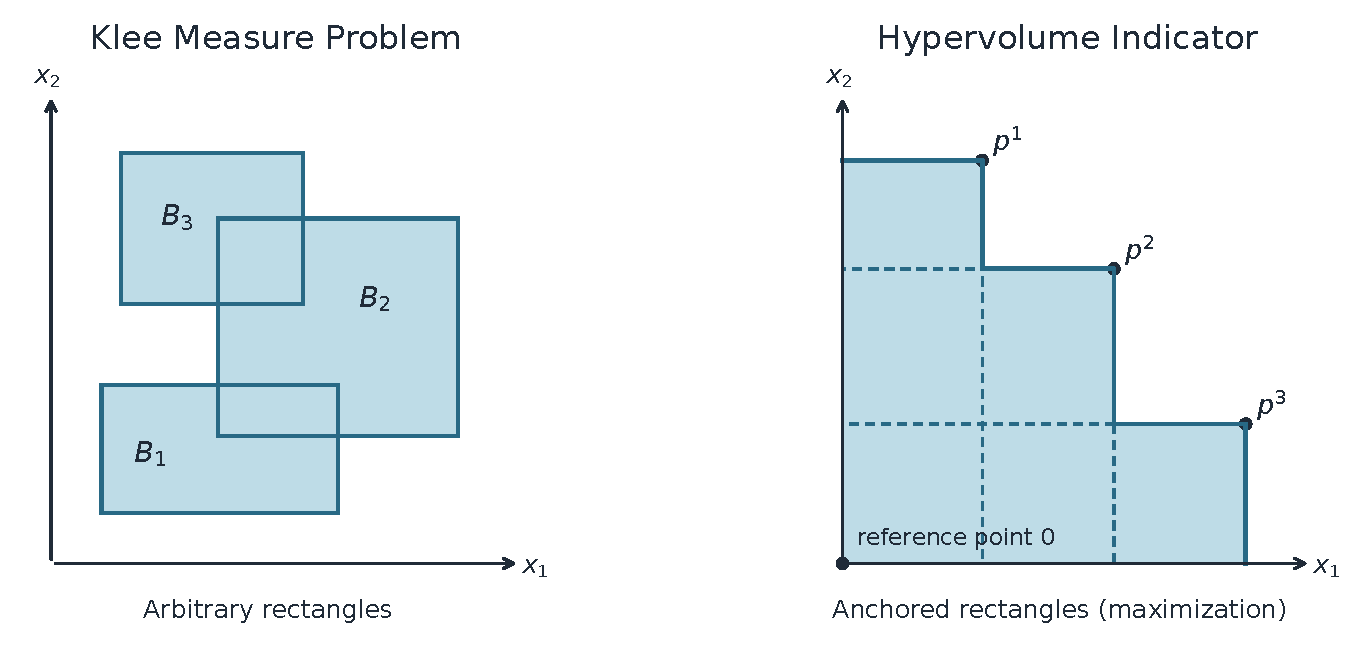
\includegraphics[width=\linewidth]{figures/klee_hypervolume_2d.pdf}
\caption{Two-dimensional instances. Left: Klee measure is the area of
the union of arbitrary axis-aligned rectangles. Right: for maximization,
the Hypervolume Indicator is the area of rectangles joining the
reference point $0$ to the objective vectors $p^1,p^2,p^3$.
The shaded union counts each overlap once.}
\label{fig:boxes}
\end{figure}

The role of the dimension requires some care. When it is fixed, exact
algorithms can have running time polynomial in the number of boxes.
When the dimension is part of the input, Bringmann and Friedrich
\cite{BringmannFriedrich} establish counting hardness even for anchored
boxes with coordinates in $\{1,2\}$. The present paper concerns a
related algebraic question. We consider computations formed from
additions and multiplications, allowing intermediate results to be
reused, and ask whether their size can be polynomially bounded.

The recent announcement of $\VP\ne\VNP$ \cite{Claude2026} prompted
this investigation. I had previously noticed a connection between
the magnitude of dominated sets and the permanent, but had not pursued
$\VNP$-hardness for these geometric quantities: with the
$\#\mathrm P$-hardness of hypervolume already
established, it seemed to add little. Transferring arithmetic lower
bounds gave this connection a new motivation.

We construct a union of anchored boxes for which the part of an
enclosing box left uncovered
represents matchings in a bipartite graph. A parameter $t$ records the
size of a matching. The residual volume is therefore a polynomial in
$t$, and its coefficient of highest possible degree is the permanent.
The row--column conflict graph and its partial-permanent polynomial
are due to Briquel and Koiran \cite{BriquelKoiran2009}. Here this
algebraic construction is realized by positive-coordinate boxes.

For an $r\times r$ matrix, the construction uses $r^2(r-1)$ boxes in
$r^2$ dimensions. The permanent is recovered from $r+1$ hypervolume
evaluations by interpolation. This reduction is unconditional.
Assuming $\VP_{\R}\ne\VNP_{\R}$, it follows that the constructed
hypervolume family has no polynomial-size arithmetic circuits. The
same conclusion applies to exact Klee measure in the stated model.
We also give the reverse reduction for rational inputs in the bit
model, and corresponding identities for ordinary $\ell_1$ magnitude.
The proofs are self-contained apart from the cited counting and
algebraic completeness theorems.

\subsection{Definitions and computational models}

Before discussing reductions, we specify what an input is and how the
cost of a computation is measured. These choices matter: counting
integer objects and evaluating a formal polynomial are related tasks,
but a lower bound for one does not automatically settle the other.

For maximization, let $P=\{p^1,\ldots,p^n\}\subseteq\R_{\ge0}^d$ and use
the reference point $0=(0,\ldots,0)$. Write
\begin{equation}
 [0,p]=\prod_{i=1}^d[0,p_i],\qquad
 D(P)=\bigcup_{p\in P}[0,p],\qquad
 \HV_d(P)=\lambda_d(D(P)).
 \label{eq:hv}
\end{equation}
Thus $D(P)$ contains the points dominated by \emph{at least one} input
vector. It is downward closed: $0\le x\le y\in D(P)$ implies $x\in D(P)$.
Klee's measure problem permits arbitrary axis-aligned boxes
$\prod_i[\ell_i,u_i]$. Hypervolume is its anchored special case.

We distinguish three measures of complexity.
\begin{enumerate}
 \item \textbf{Bit complexity.} Coordinates are integers or rationals
 encoded in binary. Running time includes operations on their bits.
 The class $\#\mathrm P$ consists of integer-valued functions that count
 accepting paths of polynomial-time nondeterministic computations.
 \item \textbf{Arithmetic circuit complexity.} A circuit uses variables,
 field constants, addition and multiplication. Negative constants permit
 subtraction. Intermediate results may be reused. The size $\size(f)$ is
 the minimum number of gates computing the \emph{formal polynomial} $f$.
 We count variable and constant gates too. Our reductions are over
 $\Q$ or $\R$; the conditional circuit lower bounds are stated over $\R$.
 \item \textbf{Representation size.} A symbolic algorithm may store
 $S$ objects called primitives. This is a complexity bound only after the
 cost of constructing and evaluating each object is specified.
\end{enumerate}

A polynomial family belongs to $\VP$ if its number of variables, degree,
and arithmetic circuit size are polynomially bounded in its index. A
family belongs to $\VNP$ if it is an exponential sum, over polynomially
many Boolean witness coordinates, of a family in $\VP$. Valiant's
completeness theorem places the permanent in $\VNP$ and makes it
$\VNP$-complete under polynomially bounded projections in characteristic
different from two \cite[Theorem 2]{ValiantAlgebra}. A projection substitutes
variables or constants. An arithmetic oracle reduction, also called a
\emph{c-reduction}, additionally permits polynomially many oracle
evaluations and arithmetic operations. Our reduction uses the latter.

\section{The permanent and the underlying field}
\label{sec:binary}

We begin with a distinction that will be used throughout the argument.
The permanent has the same defining expression over different fields,
but its computational properties depend on the arithmetic in which it
is evaluated. In particular, a matrix whose entries are zero or one
need not be a matrix evaluated over the two-element field.

The permanent of an $r\times r$ matrix is
\begin{equation}
 \per_r(A)=\sum_{\sigma\in S_r}\prod_{i=1}^r a_{i,\sigma(i)}.
 \label{eq:permanent}
\end{equation}
The determinant inserts the sign of $\sigma$ in each summand. The input
alphabet and the arithmetic used to evaluate these expressions are
separate choices.

\paragraph{A zero--one matrix evaluated over the integers.}
If $a_{ij}\in\{0,1\}$, then $\per(A)$ counts perfect matchings in the
corresponding bipartite graph. This integer-valued problem is
$\#\mathrm P$-complete \cite{ValiantCounting}. It does not become a
determinant. For example,
\begin{equation}
 A=\begin{pmatrix}1&1\\1&1\end{pmatrix}
 \quad\Longrightarrow\quad \per(A)=2,\qquad\det(A)=0.
 \label{eq:binary-example}
\end{equation}

\paragraph{A matrix evaluated in characteristic two.}
Here $-1=1$, so the signs disappear and
$\per(A)=\det(A)$. Over $\F_2$ this computes the \emph{parity} of the
matching count. Both answers in \eqref{eq:binary-example} reduce to zero.
Valiant explicitly distinguishes this case \cite[Theorem 3]{ValiantCounting}.
Our arithmetic lower-bound conclusions are over $\R$, which has
characteristic zero.

\paragraph{A formal polynomial over the reals.}
For circuit lower bounds the $a_{ij}$ are independent indeterminates.
The circuit must compute \eqref{eq:permanent} as a polynomial identity.
Agreement only on zero--one inputs is weaker: $x^2$ and $x$ agree on
$\{0,1\}$ but are distinct polynomials. Converting an arbitrary circuit
correct on the Boolean cube into a circuit for its multilinear extension
requires a separate complexity argument. A lower bound for the formal
polynomial therefore does not by itself give a lower bound for every
algorithm whose inputs are restricted to zero--one matrices. This
input restriction and the choice of characteristic are separate issues.

For our transfer, it suffices that an arithmetic circuit is correct for
all positive real parameters: two real polynomials agreeing on a
nonempty open set are identical. Positivity therefore causes no loss in
the formal-polynomial reduction.

\section{Counting complexity of hypervolume}
\label{sec:bf}

Next we recall how a volume can encode a count. The construction below
is useful background for the weighted construction later in the paper:
each small cell represents a choice, and a box covers the cells that
violate a prescribed condition. Here all relevant cells have unit
volume, so the resulting volume is an integer count.

Bringmann and Friedrich prove $\#\mathrm P$ hardness using boxes anchored
at the origin with upper corners in $\{1,2\}^d$
\cite[Theorem 1]{BringmannFriedrich}. This is already a hardness proof for
the hypervolume indicator when $d$ is part of the input.

The reduction has the following form. For a monotone CNF
$F(x)=\bigwedge_C\bigvee_{i\in C}x_i$, introduce a corner
\[
 p^C_i=\begin{cases}1,&i\in C,\\2,&i\notin C.\end{cases}
\]
Partition $[0,2]^d$, ignoring boundaries of zero volume, into the unit
cells indexed by $x\in\{0,1\}^d$. The cell for $x$ is covered by
$[0,p^C]$ precisely when every variable in $C$ is zero, so that clause
is violated. It follows that
\begin{equation}
 \HV_d(\{p^C\})=2^d-\#\{x:F(x)=1\}.
 \label{eq:bf}
\end{equation}
All counts here are integers; there is no reduction modulo two.

For this restricted family, membership in $\#\mathrm P$ follows by
guessing $x$ and testing whether its cell is covered. Together with the
hardness theorem, this gives completeness under polynomial-time
counting oracle reductions. The subtraction in \eqref{eq:bf} is part
of the reduction; it is not a parsimonious equality with the satisfying
assignment count. A polynomial-time exact bit algorithm would therefore
imply $\mathrm{FP}=\#\mathrm P$, and hence $\mathrm P=\mathrm{NP}$.
This does not supply an unconditional exponential running-time bound.
Raw rational-valued hypervolume should not itself be called a
$\#\mathrm P$ function without specifying an integer scaling convention.

\begin{table}[htbp]
\centering
\caption{Two different transfers of hardness. Both allow growing dimension.}
\label{tab:comparison}
\renewcommand{\arraystretch}{1.16}
\begin{tabularx}{\linewidth}{@{}p{0.21\linewidth}XX@{}}
\toprule
 & Counting reduction & Arithmetic reduction below\\
\midrule
Source & Number of satisfying Boolean assignments & Generic permanent polynomial\\
Coordinates & Fixed values $1$ and $2$ & Positive expressions $ta_e$ and $1+ta_e$\\
Arithmetic & Exact integer counts, encoded in bits & Formal polynomial identities over $\R$\\
Consequence & $\#\mathrm P$ hardness & Permanent circuit lower bounds transfer\\
Extra premise for an impossibility result & E.g.\ $\mathrm{FP}\ne\#\mathrm P$ & A permanent circuit lower bound\\
\bottomrule
\end{tabularx}
\end{table}

The two results complement one another. A counting reduction alone does
not establish an arithmetic circuit lower bound. Conversely, a formal
arithmetic lower bound alone does not settle the complexity of arbitrary
bit algorithms.

\section{Reductions and related algebraic constructions}
\label{sec:directions}

We now consider the relation with the permanent more closely. There
are two questions to distinguish. Can a permanent oracle be used to
compute Klee measure? Conversely, can a volume oracle be used to compute
the permanent? Both directions are meaningful, but it is the second
that transfers a permanent lower bound to volume computation. We first
explain the bit-model relation, then identify the algebraic construction
needed for the arithmetic argument.

\subsection{Klee measure reduces to the permanent in the bit model}

For binary-encoded rational endpoints, exact Klee measure is computable
using polynomially many calls to an integer permanent oracle. This is a
consequence of Valiant's counting completeness theorem
\cite[Theorem 1]{ValiantCounting}, with the following explicit additional
membership argument.

For each axis $i$, multiply all endpoints by the product $q_i$ of their
positive denominators, then translate so that all endpoints are
nonnegative integers. The resulting boxes lie in an integer bounding
box $\prod_i[0,B_i]$. Their union is, up to boundaries of zero measure,
a union of unit cells indexed by integer vectors
$z\in\prod_i\{0,\ldots,B_i-1\}$. A cell is covered precisely when
its index satisfies $\ell_i\le z_i<u_i$ on every axis for at least one
scaled input box.

The nondeterministic computation guesses the binary encoding of $z$
and accepts precisely when this test succeeds. Thus there is one
accepting witness for each covered cell, even if that cell belongs to
several boxes. The guessed
vector has polynomially many bits, and the test takes polynomial time.
The denominator products and scaled endpoints also have polynomial
bit length. Empty input and zero-volume bounding boxes return zero
directly. Thus the scaled union volume is a $\#\mathrm P$ function.
An oracle reduction to the zero--one permanent computes this integer;
division by $\prod_i q_i$ recovers the original rational volume.

This establishes
\[
 \text{rational Klee measure}\ \le_T^{\mathrm{poly}}\
 \text{integer permanent}.
\]
This bit-model reduction uses counting completeness. A global
arithmetic-circuit representation for arbitrary real box coordinates
requires a different argument.

\subsection{The opposite direction and its role in lower bounds}

The counting hardness in Section~\ref{sec:bf} already implies a
polynomial-time counting-oracle reduction in the other direction,
from the zero--one permanent to anchored Klee measure. This does not
by itself transfer lower bounds for \emph{formal polynomials}.
For that purpose, Section~\ref{sec:construction} realizes a weighted
polynomial on a positive open domain and Section~\ref{sec:transfer}
uses arithmetic interpolation. More precisely, the two steps are
\[
 \begin{aligned}
 \text{permanent polynomial}&\ \le_c\ H_r,\\
 \{\text{constructed anchored inputs}\}&\ \subseteq\
 \{\text{Klee-measure inputs}\}.
 \end{aligned}
\]
Here the last symbol denotes an inclusion of geometric instances,
not an assertion that unrestricted Klee measure is one polynomial.

\subsection{The partial permanent}

Briquel and Koiran \cite[Section 3, Theorems 3 and 5]{BriquelKoiran2009}
use a graph with one vertex for each position of an $r\times r$ matrix
and an edge between positions sharing a row or column. They identify
its independent-set polynomial with the partial permanent and establish
the relevant $\VNP$-completeness result. This is the same conflict graph
used below. With their variables replaced by $ta_e$, their polynomial
is exactly our residual $Q_r(A,t)$.

The additional step here is its geometric realization as the ambient
box volume minus the union volume of the explicit positive boxes in
\eqref{eq:corners}. We prove that step directly. The geometric construction thus extends the algebraic formulation
of Briquel and Koiran.

\section{Encoding matchings by a hypervolume residual}
\label{sec:construction}

The task is now geometric: how can a union of anchored boxes distinguish
a matching from an arbitrary selection of matrix entries? We will use
one coordinate for each permitted entry. A choice between two intervals
on that axis records whether the entry is selected. The boxes will
cover selections containing a conflict, leaving the matchings in the
complement inside an enclosing box. We first examine this mechanism
in three dimensions, where it can be drawn explicitly.

\subsection{A three-dimensional example}
\label{sec:3d-example}

Consider the matrix
\[
 A=\begin{pmatrix}a&b\\c&0\end{pmatrix},\qquad a,b,c>0.
\]
We omit the position whose entry is fixed at zero. There are therefore
three permitted positions, represented by the coordinates
$(x_a,x_b,x_c)$. Selecting both $a$ and $b$ creates a conflict in the
first row; selecting both $a$ and $c$ creates a conflict in the first
column. The entries $b$ and $c$ are compatible, since they lie in
different rows and different columns. This sparse example has three
coordinates; a general $2\times2$ matrix will require four.

For the first picture, set $a=b=c=1$ and take the enclosing cube
$C=[0,2]^3$. Split each axis at $1$. A coordinate in $[0,1]$ means
that its entry is selected, and a coordinate in $(1,2]$ means that
it is not selected. Thus the eight unit cells of $C$ represent the
eight subsets of $\{a,b,c\}$. Here these letters label matrix positions
as well as their weights. Shared cell boundaries have zero volume and
do not affect any of the calculations.

To cover the selections containing a conflicting pair, introduce
\begin{equation}
 \begin{aligned}
 B_{ab}&=[0,1]\times[0,1]\times[0,2],\\
 B_{ac}&=[0,1]\times[0,2]\times[0,1].
 \end{aligned}
 \label{eq:3d-boxes}
\end{equation}
The box $B_{ab}$ requires $a$ and $b$ to be selected and leaves the
choice of $c$ unrestricted. It therefore covers the two cells for
$\{a,b\}$ and $\{a,b,c\}$. Similarly, $B_{ac}$ covers the cells for
$\{a,c\}$ and $\{a,b,c\}$. Both boxes have the origin as a corner.
Their union volume is consequently the hypervolume indicator for the
two objective vectors $(1,1,2)$ and $(1,2,1)$, with reference point
$(0,0,0)$ and maximization.

\begin{figure}[tbp]
\centering
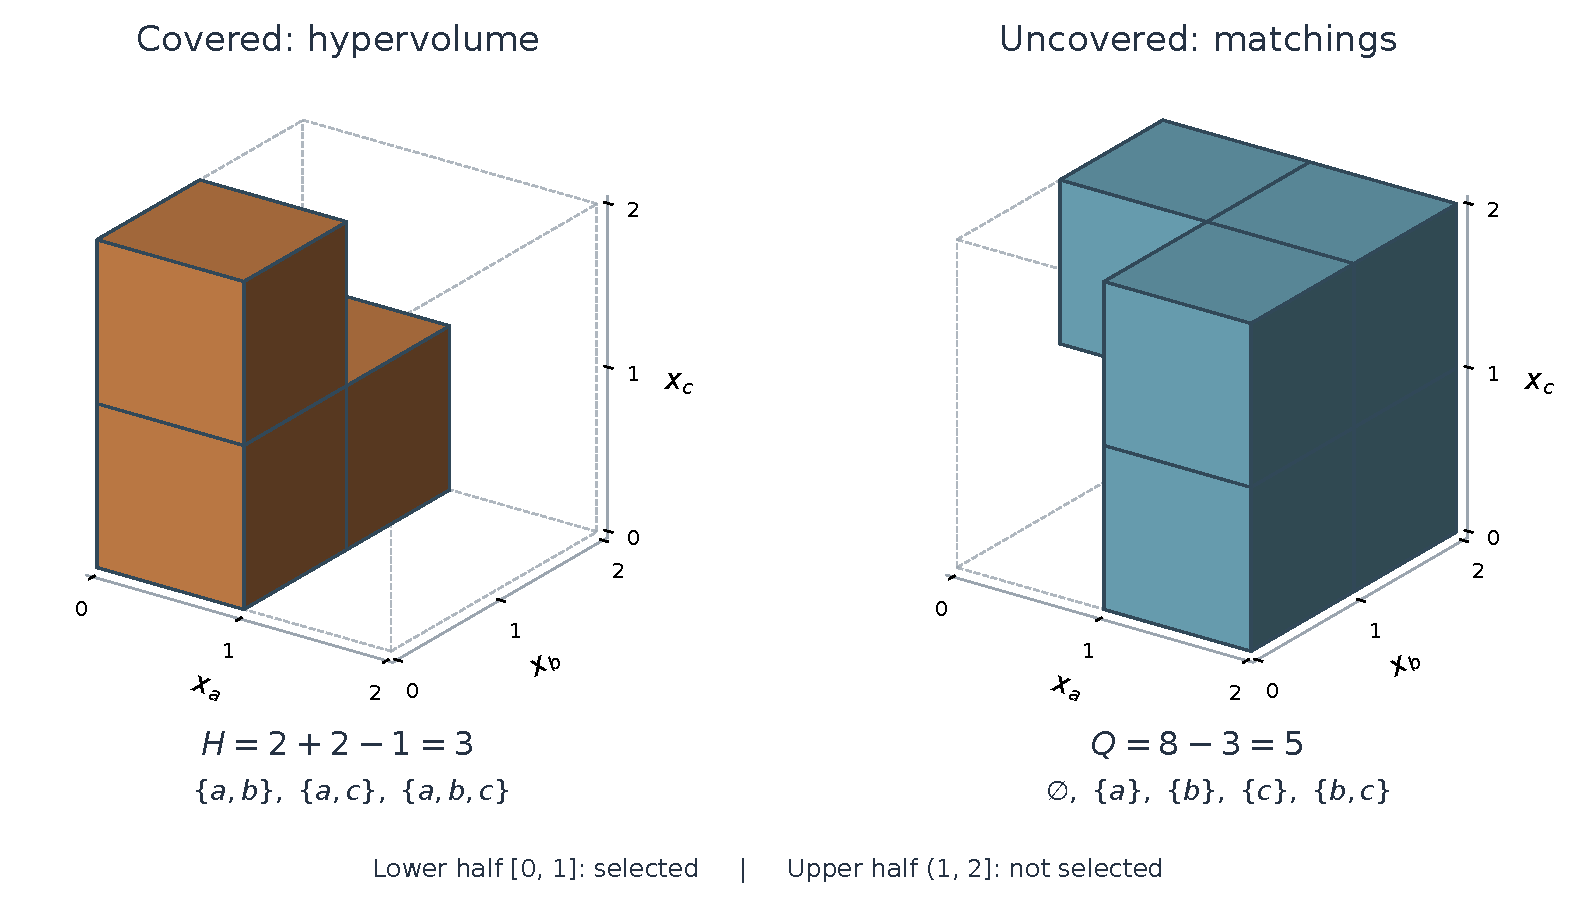
\includegraphics[width=\linewidth]{figures/hypervolume_matching_3d.pdf}
\caption{The three-dimensional matching construction in the unit case.
The orange union consists of the three cells containing a conflicting
pair. Its complement inside the same enclosing cube consists of the
five blue cells, one for each matching. A lower coordinate interval
means that the corresponding entry is selected. The two panels use
the same axes and enclosing cube.}
\label{fig:matching-3d}
\end{figure}

Each box in \eqref{eq:3d-boxes} has volume $2$, and their intersection
is the unit cube $[0,1]^3$. Hence the covered volume is
\[
 H=2+2-1=3.
\]
The uncovered volume is $Q=8-3=5$. As shown in
Figure~\ref{fig:matching-3d}, its cells represent exactly
\[
 \varnothing,\quad \{a\},\quad \{b\},\quad \{c\},\quad \{b,c\}.
\]
These are the five matchings. Only $\{b,c\}$ is perfect: it uses one
entry in each of the two rows and each of the two columns.

We now restore the weights and introduce a positive parameter $t$.
For an entry of weight $w$, replace the selected interval by $[0,tw]$
and the unselected interval by $(tw,1+tw]$. Their lengths are $tw$ and
$1$, respectively. The enclosing box and conflict boxes become
\[
 \begin{aligned}
 C(t)&=[0,1+ta]\times[0,1+tb]\times[0,1+tc],\\
 B_{ab}(t)&=[0,ta]\times[0,tb]\times[0,1+tc],\\
 B_{ac}(t)&=[0,ta]\times[0,1+tb]\times[0,tc].
 \end{aligned}
\]
The pattern of covered and uncovered cells is unchanged. The five
matching cells now have volumes $1$, $ta$, $tb$, $tc$, and $t^2bc$.
Writing $H(t)=\lambda_3(B_{ab}(t)\cup B_{ac}(t))$, we obtain
\begin{equation}
 \begin{aligned}
 Q(t)&=(1+ta)(1+tb)(1+tc)-H(t)\\
     &=1+t(a+b+c)+t^2bc.
 \end{aligned}
 \label{eq:3d-residual}
\end{equation}
The power of $t$ records how many entries have been selected. In
particular, the coefficient of $t^2$ is $bc=\per(A)$. Note that the
hypervolume query returns the covered volume $H(t)$; the matching
polynomial appears only after subtracting it from the enclosing
volume. This example explains the encoding. The lower bound will use
the same construction in a dimension that grows with the matrix size.

\subsection{The general construction}

We now keep all positions of an $r\times r$ matrix and apply the same
rule to every conflicting pair. The following notation records the
positions, their conflicts, and the resulting boxes.

Let $r\ge2$ and $E=[r]\times[r]$. We regard a matrix position
$e=(i,j)$ as an edge between row $i$ and column $j$. Distinct positions
\emph{conflict} if they share a row or a column. Let $\conf$ be the set
of unordered conflicting pairs and $\matchings$ the set of matchings,
including the empty matching.

Given positive parameters $A=(a_e)_{e\in E}$ and $t>0$, create one
coordinate for every $e\in E$. Thus the number of objectives is
$d=r^2$. For each conflicting pair $c=\{e,f\}\in\conf$, create the
corner
\begin{equation}
 p^c_g(A,t)=
 \begin{cases}
  ta_g,&g\in c,\\
  1+ta_g,&g\notin c.
 \end{cases}
 \label{eq:corners}
\end{equation}
The resulting number of corners is
\begin{equation}
 n=|\conf|=2r\binom r2=r^2(r-1).
 \label{eq:counts}
\end{equation}
No distinct positions share both their row and their column, so the two
terms in the count have no overlap. Different two-element low-coordinate
sets give opposite strict inequalities in two coordinates. Thus the
corners form an antichain: none is dominated by another.

Define the ambient box and the queried hypervolume by
\[
 C(A,t)=\prod_{e\in E}[0,1+ta_e],\qquad
 H_r(A,t)=\HV_{r^2}(\{p^c(A,t):c\in\conf\}).
\]

The ambient volume is a product of $r^2$ linear factors. Its difference
from $H_r$ measures the uncovered part of $C(A,t)$. The following
identity identifies this difference explicitly.

\begin{theorem}[Matching polynomial as residual volume]
\label{thm:matching}
For all positive $A,t$,
\begin{equation}
 \boxed{\quad
 Q_r(A,t):=\prod_{e\in E}(1+ta_e)-H_r(A,t)
   =\sum_{M\in\matchings}t^{|M|}\prod_{e\in M}a_e.
 \quad}
 \label{eq:matching}
\end{equation}
In particular,
\begin{equation}
 \deg_t Q_r\le r,\qquad [t^r]Q_r(A,t)=\per_r(A).
 \label{eq:coefficient}
\end{equation}
\end{theorem}

\begin{proof}
Partition each coordinate interval into two disjoint pieces:
\[
 [0,1+ta_e]=[0,ta_e]\;\dot\cup\;(ta_e,1+ta_e].
\]
Call the first choice selected. For $S\subseteq E$, the corresponding
product cell has volume $t^{|S|}\prod_{e\in S}a_e$, since each unselected
interval has length one.

A point in this cell lies in the box for $c=\{e,f\}$ exactly when
$e,f\in S$. The other coordinates impose no further restriction inside
$C(A,t)$. The cell avoids the union precisely when $S$ has no conflicting
pair, which means that $S$ is a matching. Summing the volumes of these
disjoint residual cells proves \eqref{eq:matching}. A matching has at
most $r$ edges, and its size is $r$ exactly when it is a perfect
matching. These matchings correspond to permutations, giving
\eqref{eq:coefficient}.
\end{proof}

Thus a cell is covered precisely when its selected positions contain
a conflicting pair. The uncovered cells correspond to matchings.
The subtraction from the ambient volume is the step that passes from
these excluded selections to the matching polynomial; the hypervolume
query itself still measures the union of anchored boxes.

\paragraph{Polynomial dependence on the parameters.}
General hypervolume is piecewise polynomial in its corner coordinates.
Here every coordinate has two levels in a fixed order,
$ta_e<1+ta_e$, on the whole positive parameter domain.
Equation~\eqref{eq:matching} therefore identifies $H_r$ with a single
polynomial in $A,t$. In the remainder, $H_r$ denotes that
polynomial as well as its geometric evaluation on positive parameters.
For interpolation, it is useful to record the degree bounds separately:
\begin{equation}
 \deg_t H_r\le r^2,\qquad \deg_{A,t}H_r\le2r^2,
 \qquad \deg_t Q_r\le r.
 \label{eq:degrees}
\end{equation}
The small degree used for interpolation belongs to the \emph{residual}
$Q_r$, after cancellation, not to the queried hypervolume $H_r$.

\subsection{A numerical example in four dimensions}

The three-dimensional picture omitted one zero entry. To see the full
construction for a matrix with all entries positive, we next give a
$2\times2$ example and compute the volumes needed for interpolation.

Take
\[
 A=\begin{pmatrix}2&3\\5&7\end{pmatrix},\qquad
 \per(A)=2\cdot7+3\cdot5=29.
\]
There are four coordinates, four conflict boxes, and seven matchings:
the empty matching, four singleton matchings and two perfect matchings.
At $t=1$, ordering coordinates as $(11,12,21,22)$, the corners are
\[
 (2,3,6,8),\quad(3,4,5,7),\quad
 (2,4,5,8),\quad(3,3,6,7).
\]
The ambient box has upper corner $(3,4,6,8)$. Directly from the matching
sum,
\[
 Q_2(A,t)=1+17t+29t^2,\qquad
 H_2(A,t)=72t^2+247t^3+210t^4.
\]
The numbers in Table~\ref{tab:example} give
$(313-2\cdot151+47)/2=29$. This illustrates the construction; it is not
an asymptotic lower bound in fixed dimension four.

\begin{table}[htbp]
\centering
\caption{Exact evaluations in the $2\times2$ example.}
\label{tab:example}
\begin{tabular}{@{}rrrr@{}}
\toprule
$t$ & Ambient volume & Hypervolume $H_2(A,t)$ & Residual $Q_2(A,t)$\\
\midrule
1 & 576 & 529 & 47\\
2 & 5775 & 5624 & 151\\
3 & 24640 & 24327 & 313\\
\bottomrule
\end{tabular}
\end{table}

\section{Transferring the arithmetic lower bound}
\label{sec:transfer}

The geometric construction has produced a polynomial whose leading
coefficient is the permanent. It remains to recover that coefficient
using only polynomially many exact volume evaluations and arithmetic
operations. The next formula does this with $r+1$ positive values of
$t$. Once the formula is available, a small circuit for the constructed
hypervolume would give a small circuit for the permanent.

\begin{lemma}[Leading coefficient from positive evaluation points]
\label{lem:interpolation}
If $q(t)$ has degree at most $r$ over a field of characteristic zero,
then
\begin{equation}
 [t^r]q(t)=\sum_{j=0}^r
       \frac{(-1)^{r-j}}{j!(r-j)!}\,q(j+1).
 \label{eq:interpolation}
\end{equation}
\end{lemma}

The formula is the $r$th forward difference at $1$, divided by $r!$.
Successive differences remove all terms of degree below $r$; the term
$t^r$ contributes $r!$. Appendix~\ref{app:interpolation} gives the
details. All query points are positive,
and the rational coefficients are permitted circuit constants. The
formula introduces no division gates. This argument is stated in
characteristic zero, where the required factorials are nonzero.

\begin{theorem}[Unconditional circuit reduction]
\label{thm:transfer}
Over $\Q$ or $\R$, the polynomial family $H_r$ defined in
Section~\ref{sec:construction} satisfies
\begin{equation}
 \boxed{\size(\per_r)\le(r+1)\size(H_r)+O(r^3).}
 \label{eq:circuit-transfer}
\end{equation}
Consequently, any superpolynomial permanent circuit lower bound transfers
to these hypervolume polynomials, with only polynomial overhead.
\end{theorem}

\begin{proof}
Use $r+1$ copies of a circuit for $H_r(A,t)$, specializing $t$ to
$1,2,\ldots,r+1$. For each value, compute
$\prod_e(1+ta_e)$ with $O(r^2)$ additional gates and subtract the
queried hypervolume. The result is $Q_r(A,t)$. Apply
\eqref{eq:interpolation}. The extra work is $O(r^3)$ in total, and
Theorem~\ref{thm:matching} identifies the output with $\per_r(A)$.
The geometric identity for positive inputs is a polynomial identity,
so the resulting circuit computes the formal permanent.
\end{proof}

Note that Theorem~\ref{thm:transfer} assumes no complexity-class
separation. It describes how to compute one polynomial from another.
The assumption $\VP_{\R}\ne\VNP_{\R}$ enters only in the following
lower-bound consequence.

\begin{corollary}[Conditional hypervolume circuit lower bound]
\label{cor:hv-lower}
If $\VP_{\R}\ne\VNP_{\R}$, the family $(H_r)$ does not have
polynomially bounded arithmetic circuit size. Equivalently,
\[
 (H_r)\notin\VP_{\R}.
\]
The obstruction is to a polynomial bound in the growing parameters
$d=r^2$, $n=r^2(r-1)$, or the dense coordinate count $nd$.
\end{corollary}

\begin{proof}
If $\size(H_r)$ were polynomially bounded in $r$,
\eqref{eq:circuit-transfer} would give polynomial-size circuits for
the permanent. Its $\VNP$-completeness over $\R$
\cite[Theorem 2]{ValiantAlgebra} would then imply
$\VP_{\R}=\VNP_{\R}$, contrary to the hypothesis.
The parameters $r,d,n,nd$ are polynomially related along this family.
\end{proof}

\begin{corollary}[Conditional Klee-measure lower bound]
\label{cor:klee}
If $\VP_{\R}\ne\VNP_{\R}$, no polynomial-size arithmetic-circuit
family computes exact Klee measure on all instances of the form
\eqref{eq:corners}. Consequently no exact arithmetic/comparison
algorithm with the operations covered in Appendix~\ref{app:branches}
has running time polynomial in both the number of boxes and the
dimension on all inputs.
\end{corollary}

Every general Klee-measure algorithm must handle these anchored
instances: their lower corners are zero. This conclusion does not
assert identical optimal dimension dependence for arbitrary-box Klee
measure and hypervolume. The class-separation assumption alone gives
no particular numerical superpolynomial rate; a stronger quantitative
premise is considered only in the discussion.

\paragraph{General position and completeness.}
Appendix~\ref{app:general-position} removes same-axis coordinate ties
with polynomially many evaluations. Appendix~\ref{app:vnp} proves that
$(H_r)$ is itself $\VNP$-complete under c-reductions in characteristic
zero.

\section{Ordinary \texorpdfstring{$\ell_1$}{l1} magnitude}
\label{sec:magnitude}

We turn next to a related measure of the dominated region. Ordinary
$\ell_1$ magnitude includes contributions from lower-dimensional
projections as well as the full-dimensional volume. At first this
suggests many separate volume computations. The aim of this section
is to show that, for the anchored unions considered here, a simple
change of upper corners combines those contributions into one
hypervolume evaluation. This also allows the permanent reduction to
be carried over to magnitude.

Equip $D(P)$ with the distance
$d_1(x,y)=\sum_i|x_i-y_i|$. Magnitude uses the similarity kernel
$k(x,y)=e^{-d_1(x,y)}$. For a finite set $X=\{x_1,\ldots,x_m\}$,
let $Z_{ij}=k(x_i,x_j)$; then
\[
 \Mag(X)=\one^{\mathsf T}Z^{-1}\one.
\]
This kernel is strictly positive definite on distinct points of
$\R^d$. For compact sets, magnitude is the supremum over finite
subsets. The definition measures metric size, not the number of
objective vectors in $P$.

For finite unions of anchored boxes, the projection formula is
\cite[Theorem 3.3]{Emmerich2026}
\begin{equation}
 \boxed{\Mag(D(P))=
 \sum_{S\subseteq[d]}2^{-|S|}\lambda_{|S|}(\pi_S D(P))
 =\mu_d(D(P)),}
 \label{eq:magnitude}
\end{equation}
where
\begin{equation}
 \mu_d=\bigotimes_{i=1}^d\left(\delta_0+\frac12\lambda\right).
 \label{eq:product-measure}
\end{equation}
For nonempty $D(P)$ the empty-subset term in \eqref{eq:magnitude} is one;
for the empty set the magnitude is zero. Appendix~\ref{app:magnitude}
gives a direct proof from the kernel, including the case of zero-length
box sides.

\subsection{The product measure and its projection terms}

The measure $\delta_0$ assigns mass one to the point $0$ and zero to
sets not containing $0$. For example,
\[
 (\delta_0+\lambda/2)([0,a])=1+a/2.
\]
In the product expansion of \eqref{eq:product-measure}, choose the
Lebesgue term in coordinates $S$ and the Dirac term outside $S$.
Integration then fixes every coordinate outside $S$ to zero. The relevant
slice is
\begin{equation}
 \{x_S:(x_S,0_{-S})\in D(P)\}=\pi_S D(P).
 \label{eq:slice}
\end{equation}
Indeed, every point in that slice is in the projection. Conversely, if
$x_S$ occurs in the projection, then $(x_S,y_{-S})\in D(P)$ for some
nonnegative $y_{-S}$. Downward closure permits replacing $y_{-S}$ by
zero. This proves \eqref{eq:slice} and explains every term of the sum.

The product measure $\mu_d$ is a positive device for evaluating magnitude
on these downsets. Its restriction to $D(P)$ is generally \emph{not} the
weighting measure whose kernel potential is one. For an interval, that
weighting measure is $(\delta_0+\delta_a+\lambda|_{[0,a]})/2$; the two
measures have the same total mass but different distributions.

\subsection{A conversion requiring one hypervolume evaluation}

\begin{proposition}[Magnitude as transformed hypervolume]
\label{prop:mag-hv}
For a finite set $P\subseteq\R_{\ge0}^d$,
\begin{equation}
 \boxed{\Mag(D(P))=
 \HV_d\bigl(\{\one+p/2:p\in P\}\bigr).}
 \label{eq:mag-hv}
\end{equation}
The reference point on the right is still zero. Only the upper corners
are transformed.
\end{proposition}

\begin{proof}
For one coordinate define $T(y)=2\max\{y-1,0\}$ on $[0,\infty)$.
The unit interval collapses to zero, contributing a unit atom, and the
remaining half-line is stretched by two. Thus the pushforward of
Lebesgue measure under $T$ is $\delta_0+\lambda/2$. Coordinatewise,
\[
 T^{-1}(D(P))=\bigcup_{p\in P}\prod_i[0,1+p_i/2].
\]
Taking volumes and using \eqref{eq:magnitude} proves the identity.
\end{proof}

There is also a reverse exact evaluation reduction with $O(nd)$
arithmetic operations and comparisons. For hypervolume, first discard
boxes with a zero side. If any boxes remain, set
$b_i=\min_{p\in P}p_i>0$, $s_i=2/b_i$, and
$p'_i=2(s_i p_i-1)$. All $p'_i\ge2$, and
\begin{equation}
 \Mag(D(P'))=\left(\prod_i s_i\right)\HV_d(P).
 \label{eq:reverse}
\end{equation}
If no boxes remain, the hypervolume is zero. Formula~\eqref{eq:reverse}
follows by applying \eqref{eq:mag-hv} and rescaling coordinates.
It is an evaluation reduction, not a global arithmetic projection in
symbolic coordinates, because selecting the $b_i$ uses minima.

Consequently, exact magnitude on these dominated sets and exact
hypervolume have closely linked numerical complexity without explicitly
computing all $2^d$ projected volumes. This does not make either problem
uniformly polynomial in the number of objectives.

\subsection{A direct arithmetic reduction for magnitude}

For the circuit statement, avoid the input-dependent scaling above.
Keep the conflict pairs from Section~\ref{sec:construction}, but use
the low and high coordinate values
\[
 \ell_e=2ta_e,\qquad L_e=2ta_e+2.
\]
Let $D^{\mathrm{mag}}_r(A,t)$ be the union of the conflict boxes with
these levels and put $G_r(A,t)=\Mag(D^{\mathrm{mag}}_r(A,t))$.

\begin{proposition}[Permanent as a magnitude residual coefficient]
\label{prop:mag-reduction}
For positive $A,t$,
\begin{align}
 R_r(A,t)
 &:=\prod_{e\in E}(2+ta_e)-G_r(A,t)\notag\\
 &=\sum_{M\in\matchings}\prod_{e\in M}(1+ta_e),
 \label{eq:mag-residual}\\
 [t^r]R_r(A,t)&=\per_r(A),\qquad \deg_t R_r\le r.
 \label{eq:mag-coefficient}
\end{align}
Hence
\begin{equation}
 \size(\per_r)\le(r+1)\size(G_r)+O(r^3).
 \label{eq:mag-transfer}
\end{equation}
If $\VP_{\R}\ne\VNP_{\R}$, the family $(G_r)$ has no
polynomially bounded arithmetic circuit size.
\end{proposition}

\begin{proof}
Under $\delta_0+\lambda/2$, the disjoint intervals
$[0,\ell_e]$ and $(\ell_e,L_e]$ have masses $1+ta_e$ and $1$.
The atom at zero is included only in the first piece. The selected
coordinates of a point in the residual again form exactly a matching.
Multiplying masses proves \eqref{eq:mag-residual}. Only perfect matchings
contribute to its coefficient of degree $r$. Apply the same interpolation
as in Theorem~\ref{thm:transfer}.
\end{proof}

Here $R_r$ is the \emph{product-measure mass} of the residual. It is not
asserted to be the intrinsic magnitude of that residual, which need not
be downward closed. Also $R_r\ne Q_r$: in the earlier numerical example,
$R_2(A,t)=7+34t+29t^2$, whereas $Q_2(A,t)=1+17t+29t^2$.
Their common leading coefficient is the permanent.

\section{Consequences for symbolic representations}
\label{sec:primitives}

A symbolic method may describe a volume by a short list of objects
rather than immediately evaluating a number. Does a short description
also give an efficient exact computation? To answer this question, we
must account for the work needed to construct the objects and to
evaluate them. The following bounds make those costs explicit.

Suppose a symbolic scheme evaluates $H_r$ exactly on the constructed
positive parameter domain. Use uniform worst-case bounds over that
domain: $B(r)$ for its construction cost in arithmetic gates, $S(r)$
for the number of final primitives, and $E(r)\ge1$ for the arithmetic
cost of evaluating each primitive from the prepared state. Assume that
assembling their values costs $O(S)$.
When all these steps admit the stated circuit simulation,
\begin{equation}
 \size(H_r)\le B(r)+O(S(r)E(r)).
 \label{eq:primitive-upper}
\end{equation}
The same assertion holds for $G_r$. Thus, conditional on
$\VP_{\R}\ne\VNP_{\R}$,
\begin{equation}
 \boxed{B(r)+S(r)E(r)\text{ is not polynomially bounded in }r.}
 \label{eq:primitive-lower}
\end{equation}
If both $B$ and $E$ are polynomially bounded, $S$ must be
superpolynomial in the worst case. This does not force every individual
input to require many primitives. Without these hypotheses, the lower bound can be
absorbed by construction or evaluation. A single object storing an
unevaluated integral or an oracle for a hard polynomial is not a
constant-cost arithmetic primitive.

\paragraph{Arithmetic comparison algorithms.}
A uniformly bounded arithmetic algorithm using addition, subtraction,
multiplication and comparisons on positive real inputs has a branch
valid on an open region. Freezing that branch produces a polynomial
circuit. Since its output agrees with $H_r$ there, it agrees identically.
Appendix~\ref{app:branches} proves this statement and extends it to
division by eliminating division gates with polynomial overhead in the
output degree. Thus comparisons and divisions do not avoid the stated
superpolynomial obstruction. For counts of rational operations, this
simulation inserts a polynomial factor into
\eqref{eq:primitive-upper}, which does not change
\eqref{eq:primitive-lower}. Operations such as bit packing and integer
rounding require a different simulation and are outside this argument.

\section{Exact algorithms and approximation}
\label{sec:limits}

To interpret the lower bound, we should place it beside known
algorithms. Two distinctions are especially relevant: whether the
dimension is fixed, and whether the answer must be exact. We discuss
these in turn, since the reduction treats growing dimension and exact
evaluation together.

\subsection{Exact algorithms and fixed dimension}

An elementary exact upper bound, valid for variable dimension, follows
from inclusion--exclusion:
\begin{equation}
 \HV_d(P)=\sum_{\varnothing\ne I\subseteq[n]}
 (-1)^{|I|+1}\prod_{k=1}^d\min_{i\in I}p^i_k.
 \label{eq:ie}
\end{equation}
Computing each subset's coordinatewise minimum from a smaller subset
gives $O(d2^n)$ arithmetic/comparison operations, after the input is
read. In rational bit
arithmetic, the arithmetic-operation count must additionally include
the cost of exact number operations.

For fixed $d$, Chan gives an $O_d(n^{d/3}\operatorname{polylog}n)$
hypervolume algorithm and an $O_d(n^{d/2})$ Klee-measure algorithm for
$d\ge3$ \cite{Chan2013}. His paper assumes constant dimension; its
notation does not specify a complete uniform dependence on $d$.

The constructed lower-bound family has $d=r^2\to\infty$. It therefore
establishes none of the following:
\begin{itemize}
 \item an $n^{4/3}$ lower bound in four dimensions, or optimality of
 Chan's exponent;
 \item an exponential-in-$d$ lower bound, or a bound of $n^{\Omega(d)}$;
 \item exclusion of every algorithm with running time $f(d)n^C$ and
 arbitrary dimension-dependent $f$.
\end{itemize}
These are different quantitative targets. On a fixed coordinate-order
region and in fixed dimension, a coordinate grid has only $O((n+1)^d)$
cells; summing its covered cell volumes already gives a polynomial-size
arithmetic expression. The lower bound here is compatible with that
fact.

\subsection{Randomized relative-error approximation}

A relative-error approximation seeks $\widehat V$ with
$\Pr[|\widehat V-V|\le\varepsilon V]\ge1-\delta$.
For boxes, the Bringmann--Friedrich union algorithm gives
$O(nd\varepsilon^{-2})$ time at constant success probability in its
arithmetic/sampling model; independent repetitions give a logarithmic
factor in $1/\delta$ \cite{BringmannFriedrich}. It applies to hypervolume
because anchored boxes are boxes.

The 2025 result on approximating Klee measure gives, for fixed $d$,
$O_d((n+\varepsilon^{-2})\log^{2d+1}n)$ time at constant success
probability. Its $\Omega(n/\varepsilon^2)$ lower bound concerns access
to general objects through volume, sampling and membership oracles,
not the full explicit corner representation of boxes
\cite{BringmannEtAl2025}. That oracle lower bound therefore does not
automatically become a lower bound for explicit hypervolume inputs.

There is no conflict with the exact reduction. Forming $Q=P-H$ subtracts
large quantities, and coefficient extraction uses signed combinations
of the resulting values. Relative error in $H$ need not give useful
relative error in $Q$ or its leading coefficient. The reduction is exact,
not approximation preserving.

\section{Discussion and conclusions}
\label{sec:discussion}

The construction links geometry and algebra through a simple rule:
cover selections containing a conflict and retain the matchings as
uncovered cells. Giving each selected interval length $ta_e$ turns
their total volume into the partial permanent. Interpolation then
recovers the permanent with polynomial overhead. Thus the geometric
identities and reductions give a precise way to transfer arithmetic
lower bounds, once such a lower bound for the permanent is assumed.

Claude (Anthropic), \emph{VP $\ne$ VNP over every field}, announced
on 23 November 2026, remains in preprint status \cite{Claude2026}.
The lower-bound corollaries above are conditional on
$\VP_{\R}\ne\VNP_{\R}$; the reductions and exact identities
are unconditional.

That preprint also states the stronger quantitative premise
\begingroup
\renewcommand*{\theHequation}{announced-permanent}
\begin{equation}
 \size_{\R}(\per_r)>
 r^{c(\log_2 r)^{1/3}}=2^{c(\log_2 r)^{4/3}}
 \quad\text{for all sufficiently large }r,
 \tag{A}\label{eq:announced}
\end{equation}
\endgroup
for some $c>0$ \cite{Claude2026}. Assuming this
specific premise, \eqref{eq:circuit-transfer} and
\eqref{eq:mag-transfer} yield
\begin{equation}
 \size_{\R}(H_r),\ \size_{\R}(G_r)
 \ge 2^{\Omega((\log r)^{4/3})}.
 \label{eq:hv-lower}
\end{equation}
Indeed, subtracting $O(r^3)$ and dividing by $r+1$ in the transfer
inequality preserves that rate. This numerical rate does \emph{not}
follow from $\VP_{\R}\ne\VNP_{\R}$ alone. The preprint's separate
approximate-circuit statement uses formal Laurent-series limits
(border complexity). This is a different notion of approximation from
the randomized relative-error volume estimates discussed above
\cite{Claude2026}.

For multiobjective optimization, the lower-bound result is primarily
of theoretical value. The Hypervolume Indicator is normally used
with a fixed number of objectives, while the number of objective
vectors may vary. In the constructed family, however, the number of
objectives is $d=r^2$ and grows with the matrix order. The result
therefore explains a limitation of exact computation when both
parameters are allowed to grow; it does not determine the best
running time for a fixed number of objectives. Improving exact
algorithms in small fixed dimensions remains a separate and
practically relevant problem.

\section*{Declaration of AI use}

AI was used for some checks, writing assistance, and drawing the example
figure. The author developed the mathematical derivations, the text,
and the proofs.

\appendix
\section{The coefficient-extraction identity}
\label{app:interpolation}

Let $\Delta q(t)=q(t+1)-q(t)$. If $q$ has degree $k\ge1$ and leading
coefficient $a_k$, then $\Delta q$ has degree $k-1$ and leading
coefficient $ka_k$. Repeating this operation $r$ times kills every
monomial of degree less than $r$ and sends $t^r$ to $r!$. Thus
\[
 \Delta^r q(1)=r![t^r]q(t).
\]
Expanding the repeated difference gives
\[
 \Delta^r q(1)=\sum_{j=0}^r(-1)^{r-j}\binom rj q(1+j).
\]
Division by $r!$ yields Lemma~\ref{lem:interpolation}. The fractions
are fixed rational constants, depending only on $r$. This distinction
matters: multiplying by a constant such as $1/r!$ is allowed in a
division-free circuit over $\Q$ or $\R$.

For positive rational matrix entries and the integer query points used here,
the coordinates also have polynomial encoding length. The construction
therefore provides a polynomial-time exact numerical oracle reduction
in the bit model as well. That fact alone does not transfer an
arithmetic circuit lower bound to arbitrary bit algorithms.

\section{Removing coordinate ties exactly}
\label{app:general-position}

Coordinate general position means that, on each axis, different upper
corners have different coordinate values. The unperturbed construction
has two levels on each axis, so it does not satisfy that condition.

Enumerate the $n$ conflict boxes as $c=1,\ldots,n$ and set
\begin{equation}
 p^c_g(A,t,\eta)=p^c_g(A,t)+\eta\frac{c}{n+1},
 \qquad 0<\eta<1.
 \label{eq:perturbation}
\end{equation}
Within each level the coordinates are now distinct. A low coordinate
is still strictly less than every high coordinate on the same axis,
because the original gap is one and the perturbation difference has
absolute value less than one. Positivity and the antichain property
are preserved. The ordering depends only on the low/high pattern and
the index $c$, not on $A,t,\eta$ in this domain.

Let $H_r^\eta(A,t)$ be the perturbed hypervolume. Apply
\eqref{eq:ie}. On this fixed ordering, each coordinatewise minimum in
each term is a fixed affine expression in $\eta$. A product has at most
$d$ such factors, so the whole result is a polynomial in $\eta$ of
degree at most $d=r^2$. It is also a polynomial in the other parameters.
Its value at $\eta=0$ is the original $H_r(A,t)$.

Choose $d+1$ distinct constants in $(0,1)$, for example
$\eta_k=k/(d+2)$, $k=1,\ldots,d+1$. Lagrange interpolation gives
\begin{equation}
 H_r(A,t)=\sum_{k=1}^{d+1}\gamma_k H_r^{\eta_k}(A,t),
 \qquad
 \gamma_k=\prod_{\substack{1\le h\le d+1\\h\ne k}}
             \frac{-\eta_h}{\eta_k-\eta_h}.
 \label{eq:eta-interpolation}
\end{equation}
The constants $\gamma_k$ are rational and independent of $A,t$.

For each $t=1,\ldots,r+1$, first recover the unperturbed $H_r(A,t)$
using \eqref{eq:eta-interpolation}, then form $Q_r(A,t)$, and only then
apply Lemma~\ref{lem:interpolation} in $t$. This uses
$(r+1)(d+1)=O(r^3)$ geometric queries and polynomial extra work. Hence
the circuit and arithmetic/comparison lower bounds survive coordinate
general position with polynomial overhead.

\paragraph{Order of coefficient extraction.}
The perturbed boxes can extend beyond the original ambient box
$C(A,t)$. Moreover,
$\prod_e(1+ta_e)-H_r^\eta(A,t)$ need not have degree at most $r$ in
$t$. It cannot be given the original matching-residual interpretation.
One must recover $\eta=0$ before using the degree-$r$ cancellation.
The same perturbation argument applies to the magnitude family by
Proposition~\ref{prop:mag-hv}; its low/high gap is two before the corner
transformation.

\section{A formal \texorpdfstring{$\VNP$}{VNP} classification}
\label{app:vnp}

We prove membership without treating a geometric integration operation
as an arithmetic gate. For $z\in\{0,1\}^{E}$ define the polynomials
\begin{align*}
 w(z,A,t)&=\prod_{e\in E}(1-z_e+z_e ta_e),\\
 b(z)&=1-\prod_{\{e,f\}\in\conf}(1-z_ez_f).
\end{align*}
On Boolean $z$, $b(z)$ is one if the selected positions contain a
conflict, and zero otherwise. The value of $w$ is the volume of the
corresponding cell. Therefore
\begin{equation}
 H_r(A,t)=\sum_{z\in\{0,1\}^{r^2}}w(z,A,t)b(z).
 \label{eq:vnp-witness}
\end{equation}
The summand has an $O(r^3)$-size circuit, a polynomial number of
variables, and polynomial degree, so it is a $\VP$ family. This is
exactly a $\VNP$ witness for $H_r$.

Theorem~\ref{thm:transfer} gives an arithmetic oracle reduction from
the permanent to $H_r$. Combining it with Valiant's permanent
completeness theorem \cite{ValiantAlgebra} shows that $(H_r)$ is
$\VNP$-complete under c-reductions over characteristic zero. The
interpolation step is why the stated reduction notion is c-reduction,
not projection.

This classification concerns the explicit polynomial family $H_r$.
It does not put the unrestricted, globally piecewise-polynomial
hypervolume map into a class whose objects are single polynomials.

\section{A direct proof of the magnitude formula}
\label{app:magnitude}

This appendix proves \eqref{eq:magnitude} from the similarity kernel
rather than assuming additivity of magnitude for arbitrary unions.
All sets here are compact finite unions of anchored boxes.

\subsection{Interval and box weighting measures}

For $a\ge0$ define the finite measure
\[
 w_a=\tfrac12\delta_0+\tfrac12\delta_a
                   +\tfrac12\lambda|_{[0,a]}.
\]
When $a=0$ the half-atoms combine into $\delta_0$. Direct integration,
separating $0\le x\le a$ and $x\ge a$, gives
\begin{equation}
 \int e^{-|x-y|}\,dw_a(y)=e^{-(x-a)_+},\qquad x\ge0,
 \label{eq:interval-potential}
\end{equation}
where $u_+=\max\{u,0\}$. In particular the potential is one on
$[0,a]$, and the total mass is $1+a/2$.

For a box $[0,p]$, set $w_p=\bigotimes_iw_{p_i}$. The factorization
$e^{-\|x-y\|_1}=\prod_i e^{-|x_i-y_i|}$ implies
\begin{equation}
 \int e^{-\|x-y\|_1}\,dw_p(y)
       =\exp\!\left(-\sum_i(x_i-p_i)_+\right),
 \label{eq:box-potential}
\end{equation}
and $w_p([0,p])=\prod_i(1+p_i/2)$.

\subsection{A weighting measure for an anchored union}

Let $P=\{p^1,\ldots,p^n\}$ be nonempty. For nonempty
$I\subseteq[n]$, write $p^I=\bigwedge_{i\in I}p^i$ for the coordinatewise
minimum. The intersection of the corresponding anchored boxes is
$[0,p^I]$. Define the finite signed measure
\begin{equation}
 w_D=\sum_{\varnothing\ne I\subseteq[n]}(-1)^{|I|+1}w_{p^I}.
 \label{eq:union-weight}
\end{equation}
Its support lies in $D=D(P)$.

Fix $x\in D$ and choose $j$ such that $x\le p^j$. Pair every nonempty
$I\subseteq[n]\setminus\{j\}$ with $I\cup\{j\}$. Their potentials
from \eqref{eq:box-potential} agree, since for each coordinate $k$,
\[
 (x_k-\min\{p^I_k,p^j_k\})_+=(x_k-p^I_k)_+.
\]
The signs of the two terms are opposite. All paired terms cancel,
and the remaining singleton $\{j\}$ has potential one. Hence
\begin{equation}
 \int_D e^{-\|x-y\|_1}\,dw_D(y)=1\qquad(x\in D).
 \label{eq:potential-one}
\end{equation}

\subsection{Identification of magnitude from the potential}

For finite signed measures on $D$, define the energy
\[
 \mathcal E(\nu,\rho)=\iint_D e^{-\|x-y\|_1}\,d\nu(x)\,d\rho(y).
\]
Positivity of this bilinear form follows, for example, by taking
products of the elementary Fourier identity
\[
 e^{-|u-v|}=\frac1\pi\int_{\R}
                  \frac{e^{i\xi(u-v)}}{1+\xi^2}\,d\xi.
\]
For finitely supported nonzero measures on distinct points, the energy
is strictly positive. Cauchy--Schwarz therefore applies. From
\eqref{eq:potential-one},
\[
 \mathcal E(\nu,w_D)=\nu(D),\qquad
 \mathcal E(w_D,w_D)=w_D(D).
\]
Consequently, for every nonzero finitely supported signed $\nu$,
\begin{equation}
 \frac{\nu(D)^2}{\mathcal E(\nu,\nu)}\le w_D(D).
 \label{eq:energy-bound}
\end{equation}
For a finite support $X$ with similarity matrix $Z$, maximizing the
left side over its weight vectors gives
$\one^{\mathsf T}Z^{-1}\one$ by Cauchy--Schwarz in the inner product
defined by $Z$. Its supremum over finite supports is therefore the
definition of $\Mag(D)$.

For the reverse inequality, partition compact $D$ into sets of diameter
tending to zero, and move the signed mass of each cell to a
representative in that cell. The resulting finitely supported measures
$\nu_m$ have the same total mass as $w_D$, uniformly bounded total
variation, and energies converging to $\mathcal E(w_D,w_D)$ by uniform
continuity of the kernel. Moreover $w_D(D)>0$: this follows directly
from the inclusion--exclusion mass computation in the next paragraph,
since $D$ contains the origin and $\mu_d$ has a unit atom there. Taking
limits in the variational quotient proves $\Mag(D)=w_D(D)$.

\subsection{Computing the mass and the projection terms}

The total mass of \eqref{eq:union-weight} is
\begin{align*}
 w_D(D)
 &=\sum_{\varnothing\ne I\subseteq[n]}(-1)^{|I|+1}
                \prod_k(1+p^I_k/2)\\
 &=\sum_{\varnothing\ne I\subseteq[n]}(-1)^{|I|+1}
                \mu_d([0,p^I])
 =\mu_d(D).
\end{align*}
The final equality is inclusion--exclusion for the positive measure
$\mu_d$, not an assumption about magnitude. Expanding its product
and using the slice equality \eqref{eq:slice} gives the projection sum
in \eqref{eq:magnitude}. The empty union has zero measure and magnitude
by definition. This completes the proof, including degenerate boxes.

\section{When an arithmetic comparison algorithm yields a circuit}
\label{app:branches}

\begin{lemma}[An open branch]
\label{lem:branch}
Let $U\subseteq\R^k$ be nonempty and open. Suppose a deterministic
algorithm is correct on all of $U$, uses real constants and only
addition, subtraction, multiplication and comparisons, and has a
uniform bound $T$ on the number of operations there. If its output is
a polynomial $f$ on $U$, then $f$ has an arithmetic circuit with
$O(T+k)$ gates.
\end{lemma}

\begin{proof}
For fixed input length the depth bound gives finitely many possible
execution branches. Along any one branch all computed quantities are
polynomials in the input. Gather the finitely many polynomials compared
on all branches, after subtracting the two sides of each comparison.
Discard the identically zero polynomials. The union of the zero sets of
the remaining polynomials has empty interior, so there is a point of
$U$ outside this union. In a sufficiently small neighborhood of this
point all their signs stay fixed. Identically zero comparisons also
have fixed outcomes. The algorithm therefore follows a single branch
throughout that neighborhood.

Freeze that branch and retain its arithmetic operations, replacing
subtraction by addition and multiplication by $-1$ as needed. Its output
is a polynomial $g$ computed with $O(T+k)$ gates. Correctness gives
$g=f$ on a nonempty open set, hence as a polynomial identity.
\end{proof}

To apply the lemma to a general hypervolume algorithm, compose its
input with \eqref{eq:corners}. These coordinates are polynomial
expressions in the $r^2+1$ positive parameters, so the lemma applies
on that parameter domain. If the algorithm is only promised coordinate
general position, use \eqref{eq:perturbation} and the interpolation in
Appendix~\ref{app:general-position}. Polynomial input-construction
overhead does not change the superpolynomial consequence.

This is a worst-case, nonuniform circuit argument: the good branch
need not be found efficiently. It covers arbitrary real constants and
sharing of computed values. It does not automatically cover algorithms
whose non-arithmetic operations have not been simulated, nor algorithms
required to work only on a finite Boolean input set.

\subsection{Allowing division with polynomial overhead}

Suppose division is also permitted, with denominators nonzero whenever
the relevant operation is executed, and the output polynomial $f$ has
degree at most $D$. The open-branch argument still applies: along a
branch all quantities are rational functions, and one avoids the zero
sets of their nonzero numerators and denominators. Freeze a branch
valid on an open region, and choose a point $a$ in that region where all
executed divisions are defined. The resulting rational expression agrees
with $f$ on an open set and hence as a rational-function identity.

Substitute $X=a+s(Y-a)$, where $s$ is a new formal parameter. Compute
the coefficients through degree $D$ in $s$ at every gate. Addition and
truncated multiplication use respectively $O(D+1)$ and $O((D+1)^2)$
arithmetic gates. At a division gate, the denominator has series
$u(s)=u_0+u_1s+\cdots$ with $u_0\ne0$, since its value at $a$ is
nonzero. Its inverse coefficients are obtained from
\[
 v_0=u_0^{-1},\qquad
 v_k=-u_0^{-1}\sum_{i=1}^k u_i v_{k-i}\quad(1\le k\le D).
\]
Here $u_0^{-1}$ is a fixed field constant, so no variable division is
used. Multiplication by this inverse implements the division gate
modulo $s^{D+1}$ with $O((D+1)^2)$ gates.

The output is the truncated series of $f(a+s(Y-a))$. This polynomial
has degree at most $D$ in $s$, so truncation loses nothing at the output.
Adding its coefficient polynomials, which is evaluation at $s=1$,
recovers $f(Y)$. The entire division-free circuit has size
$O((T+k)(D+1)^2)$. No bound on intermediate rational-function degrees
is required. For $H_r$ and $G_r$ we can take $D\le2r^2$, so this
overhead is polynomial in $r$ and preserves the transferred
superpolynomial lower bound for exact arithmetic/comparison algorithms
that also use division.

\clearpage
\begin{thebibliography}{99}
\interlinepenalty=10000

\bibitem{ValiantCounting}
Leslie G. Valiant.
The complexity of computing the permanent.
\emph{Theoretical Computer Science} 8(2):189--201, 1979.
\href{https://doi.org/10.1016/0304-3975(79)90044-6}{doi:10.1016/0304-3975(79)90044-6}.
\href{https://sites.math.washington.edu/~billey/colombia/references/valiant.permanent.1979pdf.pdf}{University-hosted scan}.

\bibitem{ValiantAlgebra}
Leslie G. Valiant.
Completeness classes in algebra.
In \emph{Proceedings of the Eleventh Annual ACM Symposium on Theory of
Computing (STOC '79)}, pp.~249--261, 1979.
\href{https://doi.org/10.1145/800135.804419}{doi:10.1145/800135.804419}.
\href{https://sites.math.washington.edu/~billey/colombia/references/valiant.completeness.1979.pdf}{University-hosted scan}.

\bibitem{BringmannFriedrich}
Karl Bringmann and Tobias Friedrich.
Approximating the volume of unions and intersections of high-dimensional
geometric objects.
\emph{Computational Geometry} 43(6--7):601--610, 2010.
\href{https://doi.org/10.1016/j.comgeo.2010.03.004}{doi:10.1016/j.comgeo.2010.03.004}.
\href{https://people.mpi-inf.mpg.de/~kbringma/paper/J2010CGTA.pdf}{Author manuscript}.

\bibitem{BriquelKoiran2009}
Ir\'en\'ee Briquel and Pascal Koiran.
A dichotomy theorem for polynomial evaluation.
In \emph{Mathematical Foundations of Computer Science 2009 (MFCS)},
pp.~187--198, 2009.
\href{https://doi.org/10.1007/978-3-642-03816-7_17}{doi:10.1007/978-3-642-03816-7\_17}.
\href{https://perso.ens-lyon.fr/pascal.koiran/Publis/mfcs09.dichotomy_theorem.pdf}{Author manuscript}.

\bibitem{Chan2013}
Timothy M. Chan.
Klee's measure problem made easy.
In \emph{2013 IEEE 54th Annual Symposium on Foundations of Computer
Science (FOCS)}, pp.~410--419, 2013.
\href{https://doi.org/10.1109/FOCS.2013.51}{doi:10.1109/FOCS.2013.51}.
\href{https://tmc.web.engr.illinois.edu/easyklee8_13.pdf}{Author manuscript}.

\bibitem{BringmannEtAl2025}
Karl Bringmann, Kasper Green Larsen, Andr\'e Nusser, Eva Rotenberg,
and Yanheng Wang.
Approximating Klee's measure problem and a lower bound for union volume
estimation.
In \emph{41st International Symposium on Computational Geometry
(SoCG 2025)}, LIPIcs 332, pp.~25:1--25:16, 2025.
\href{https://doi.org/10.4230/LIPIcs.SoCG.2025.25}{doi:10.4230/LIPIcs.SoCG.2025.25}.
\href{https://drops.dagstuhl.de/entities/document/10.4230/LIPIcs.SoCG.2025.25}{Publisher record and full text}.

\bibitem{Emmerich2026}
Michael T. M. Emmerich.
\emph{The Magnitude of Dominated Sets: A Pareto Compliant Indicator
Grounded in Metric Geometry}.
Preprint, arXiv:2604.18147v1, 20 April 2026.
\href{https://doi.org/10.48550/arXiv.2604.18147}{doi:10.48550/arXiv.2604.18147}.
\href{https://arxiv.org/html/2604.18147v1}{Version 1 full text}.

\bibitem{Claude2026}
Claude (Anthropic).
\emph{VP $\ne$ VNP over every field}.
Preprint, version 1, 23 November 2026.
\href{https://hexagonmath.org/2611.00954v1}{Versioned primary posting at Hexagon}.
\href{https://github.com/anthropics/formal-math/tree/11b6c7e3c927df2658f513b6b68ea7f8929c62c5/vp-vnp}{Paper and Lean formalization}.

\end{thebibliography}
\end{document}
